\documentclass[english]{mlutalk}
% \documentclass[english,handout]{mlutalk}

\title{Grimjack at Touché 2022}
\subtitle{Advanced IR, Winter Semester 2021/22}
\author{Johannes Huck \and Jan Heinrich Reimer}
\institute{Martin Luther University Halle-Wittenberg}
\date{\today}
\titlegraphic{
\includegraphics[width=3cm]{figures/mlu-halle}}

\addbibresource{../literature/literature.bib}

\usetikzlibrary{positioning}
\usepackage{listings}
\usepackage{xspace}
\usepackage{tabularx}
\usepackage{booktabs}

\newcommand{\TF}{\mbox{TF}\xspace}
\newcommand{\TFIDF}{\mbox{TF/IDF}\xspace}
\newcommand{\todocite}{{\smaller\color{red}[CITE]}\xspace}
\newcommand{\todo}[1]{{\smaller\color{red}[#1]}}

\lstset{%
  basicstyle=\ttfamily,
  breaklines=true
}

\begin{document}

\titleframe

\begin{frame}{Task at hand}  
  \begin{itemize}
    \item Task 2 of Touché: Argument Retrieval
    \item Argument Retrieval for Comparative Questions
    \item Task: Retrieve relevant passages to answer comparative questions and detect their stance w.r.t the objects
    \item Data: > 1 million text passages  
  \end{itemize}
  \begin{figure}
      \centering
      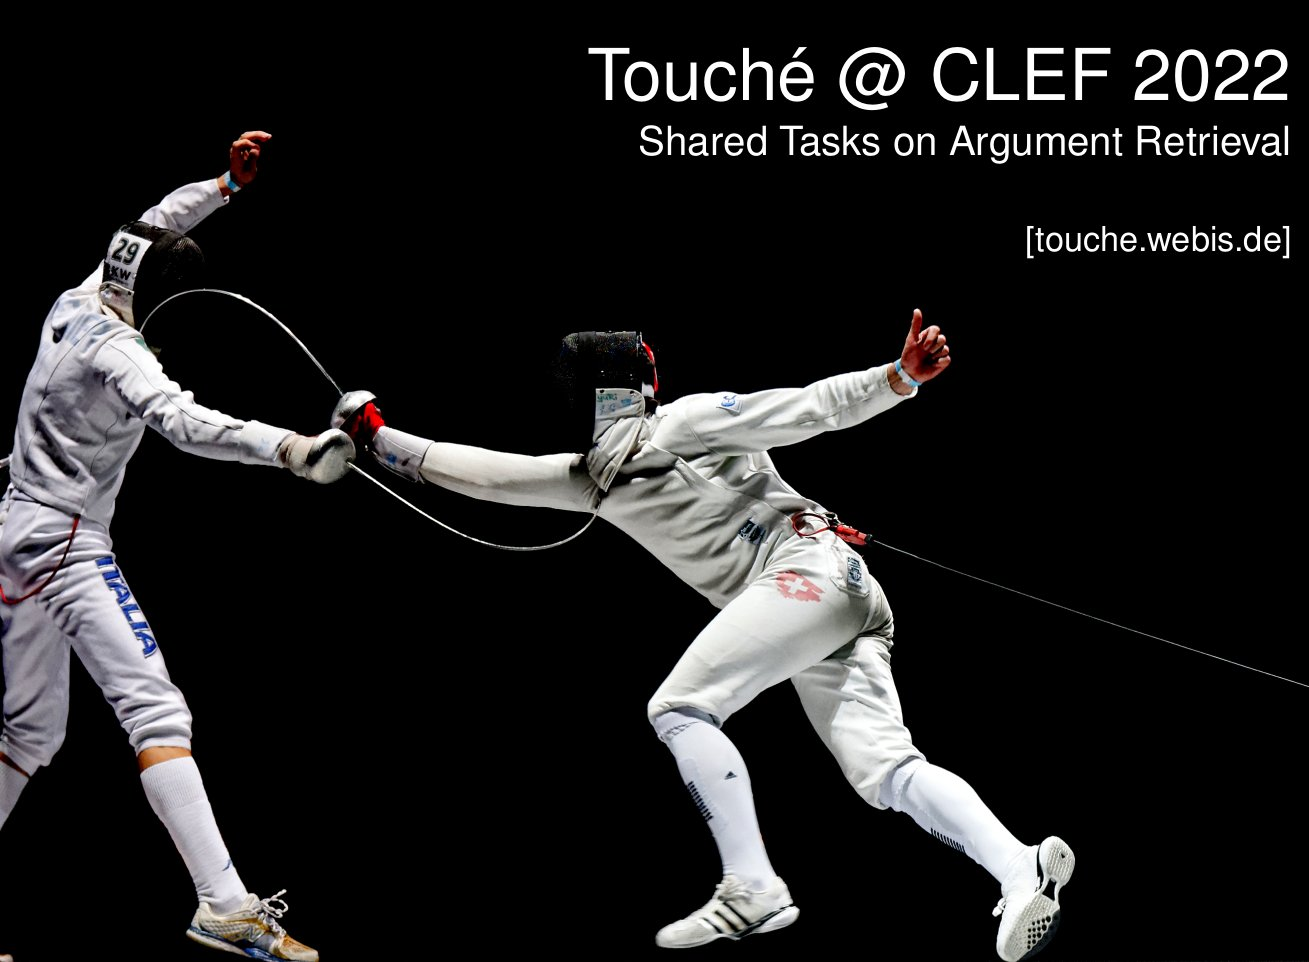
\includegraphics[height=4.8cm, width=8cm]{figures/touche}\\
      \begin{footnotesize}
        \url{https://mobile.twitter.com/webis_de/status/1468529926026534913?cxt=HHwWgoC97fyLouEoAAAA}
      \end{footnotesize}  
  \end{figure}
\end{frame}

\begin{frame}{General approach}
  \begin{itemize}
    \item Programmed in Python
    \begin{itemize}
        \item Easy to use
        \item High readability
        \item Many IR libabries available
    \end{itemize}
    \item Three modules: Search, Run file  and Evaluate
    \item Pipeline consists of
    \begin{itemize}
        \item Query-Expander and Query-Combiner
        \item Initial Retrieval
        \item Argument quality and stance tagging
        \item Reranking
    \end{itemize}
    \item Indexing and initial retrieval via pyserini~\cite{LinMLYPN2021}
  \end{itemize}
\end{frame}

\begin{frame}{Pipeline}
    \begin{figure}
        \centering
        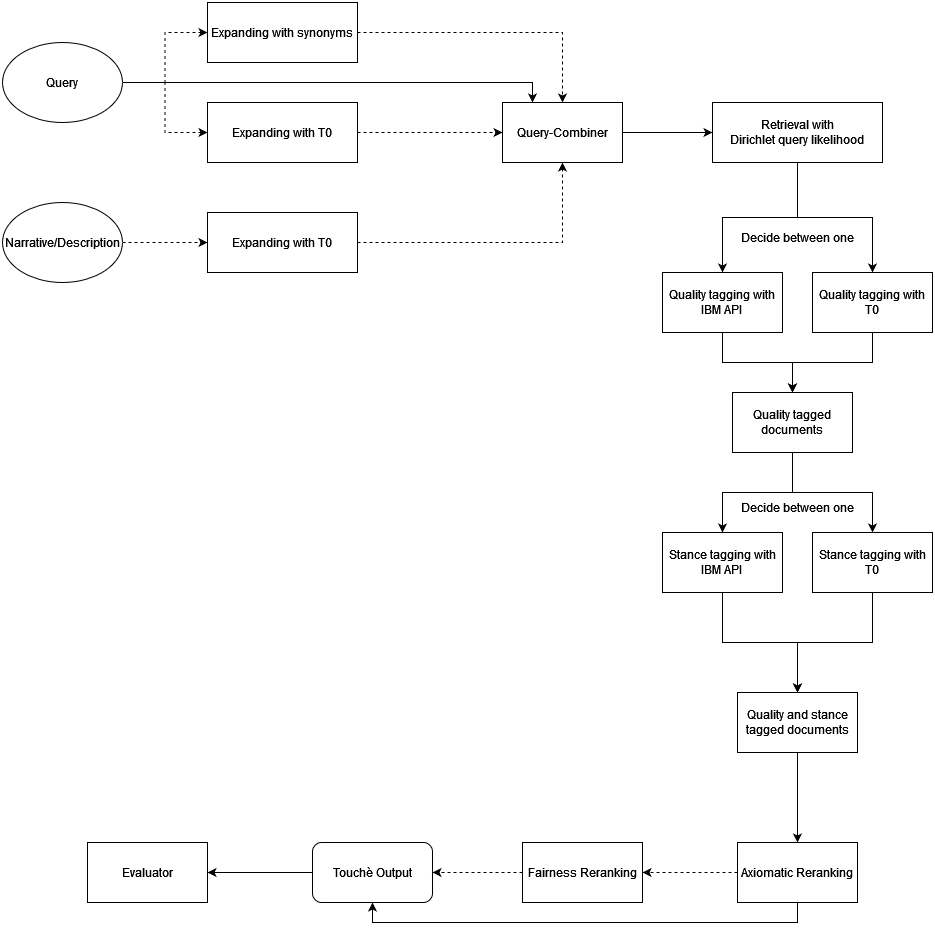
\includegraphics[scale=0.25]{figures/pipeline}
    \end{figure}
\end{frame}

\begin{frame}{Query-Expander and Query-Combiner}
    \begin{itemize}
        \item Expanding queries with synonyms of comparative objects
        \item Two Different approaches
        \begin{itemize}
            \item Based on embeddings with glove
            \item Based on language model T0~\cite{SanhWRBSACSLRDBXTSSKCNDCJWMSYPBWNRSSFFTBGBWR2021}
            \item We ask "What are synonyms of the word <token> ?" 
        \end{itemize}
        \item With T0 also new queries from narrative and description
        \item We ask "<text> Extract a natural search query from this description."
        \item Combining all new queries with OR
        \item Retrieving ranked list of passages with this new query 
    \end{itemize}
\end{frame}

\begin{frame}{Argument quality tagging}
    \begin{itemize}
        \item Extracting arguments with TARGER~\cite{ChernodubOHBHBP2019}
        \item For each argument we want to know the quality w.r.t. the topic
        \item Two different approaches
        \begin{itemize}
            \item Based IBM Debater API~\cite{ToledoG2019}
            \item Based on T0
            \item We ask "<sentence>
            How would you rate the readability and consistency in this sentence? very good, good, bad, very bad"
        \end{itemize}
        \item IBM API returns a score between 0 and 1
        \item 0 means lowest quality and 1 highest quality
    \end{itemize}
    \begin{block}{Example}
        Arg: Cars should only provide assisted driving, not complete autonomy\\
        Topic: We should further explore the development of autonomous vehicles\\
        Score: 0.7256
    \end{block}
\end{frame}

\begin{frame}{Argument stance tagging}
    \begin{itemize}
        \item Next we want to know the stance w.r.t. the topic
        \item Two different approaches
        \begin{itemize}
            \item Based on IBM Debater API~\cite{BarHaimBDSS2017}
            \item Based on T0
            \item We ask "<sentence> Is this sentence pro/against <comparative\_object>? yes or no"
        \end{itemize}
        \item It is also possible to expand with sentiments
        \item Both approaches only work for single target stance
        \item Calculating the multi target stance
        \begin{itemize}
            \item Calculate the difference between objects
            \item Use a threshold
            \item Convert T0s output into a numerical representation
        \end{itemize}
    \end{itemize}
\end{frame}

\begin{frame}{Reranking}
    \begin{itemize}
        \item Foo
    \end{itemize}
\end{frame}

\begin{frame}{Final Remarks}
    \begin{itemize}
        \item Approach is very flexible 
        \item We investigate influence of components w.r.t the retrieval score
        \item Stance classification may be better with Roberta approach
        \item We cannot distinguish between neutral and no stance
        \item We investigate how reranking influences the retrieval score
        \item T0 solves a lot of IR tasks
        \item Is it possible to only use T0 for retrieval?
    \end{itemize}
    \thankyou
\end{frame}

\appendix
\section{\appendixname}

\bibliographyframe

\end{document}